% Provenance (never printed): old seconde/premiere S material on the water
% cycle on land (the drainage basin, river discharge, floods and their
% management); see sources/book2/PROVENANCE.md. The Varden basin is computed
% in figdata/grade-10/varden_basin.py from figdata/shared/region.py; the
% Potomac record in figdata/grade-10/flood_frequency.py.
\chapter{Cuencas hidrográficas, ríos y crecidas}\label{ch:g10:drainage-basins}

Un río puede crecer dos días después de que haya dejado de llover, en una
ciudad donde no ha caído ni una gota. El agua que inunda sus calles cayó
antes, sobre colinas muy aguas arriba; bajó por sus laderas hasta los
arroyos, y los arroyos se juntaron en el río que la llevó, toda a la vez,
hasta la ciudad. Para entender una crecida hay que mirar más allá del río,
a toda la superficie que lo alimenta, y seguir el agua a través de ella. Este
capítulo define esa superficie, la \omterm{def:g10:drainage-basins:drainage-basin}{cuenca hidrográfica}; mide lo que lleva un
río, su \omterm{def:g10:drainage-basins:discharge}{caudal}; sigue una crecida a su paso por un punto del río, y muestra
cómo un registro largo de crecidas indica con qué frecuencia vuelve una
crecida dada.

\begin{omfigure}
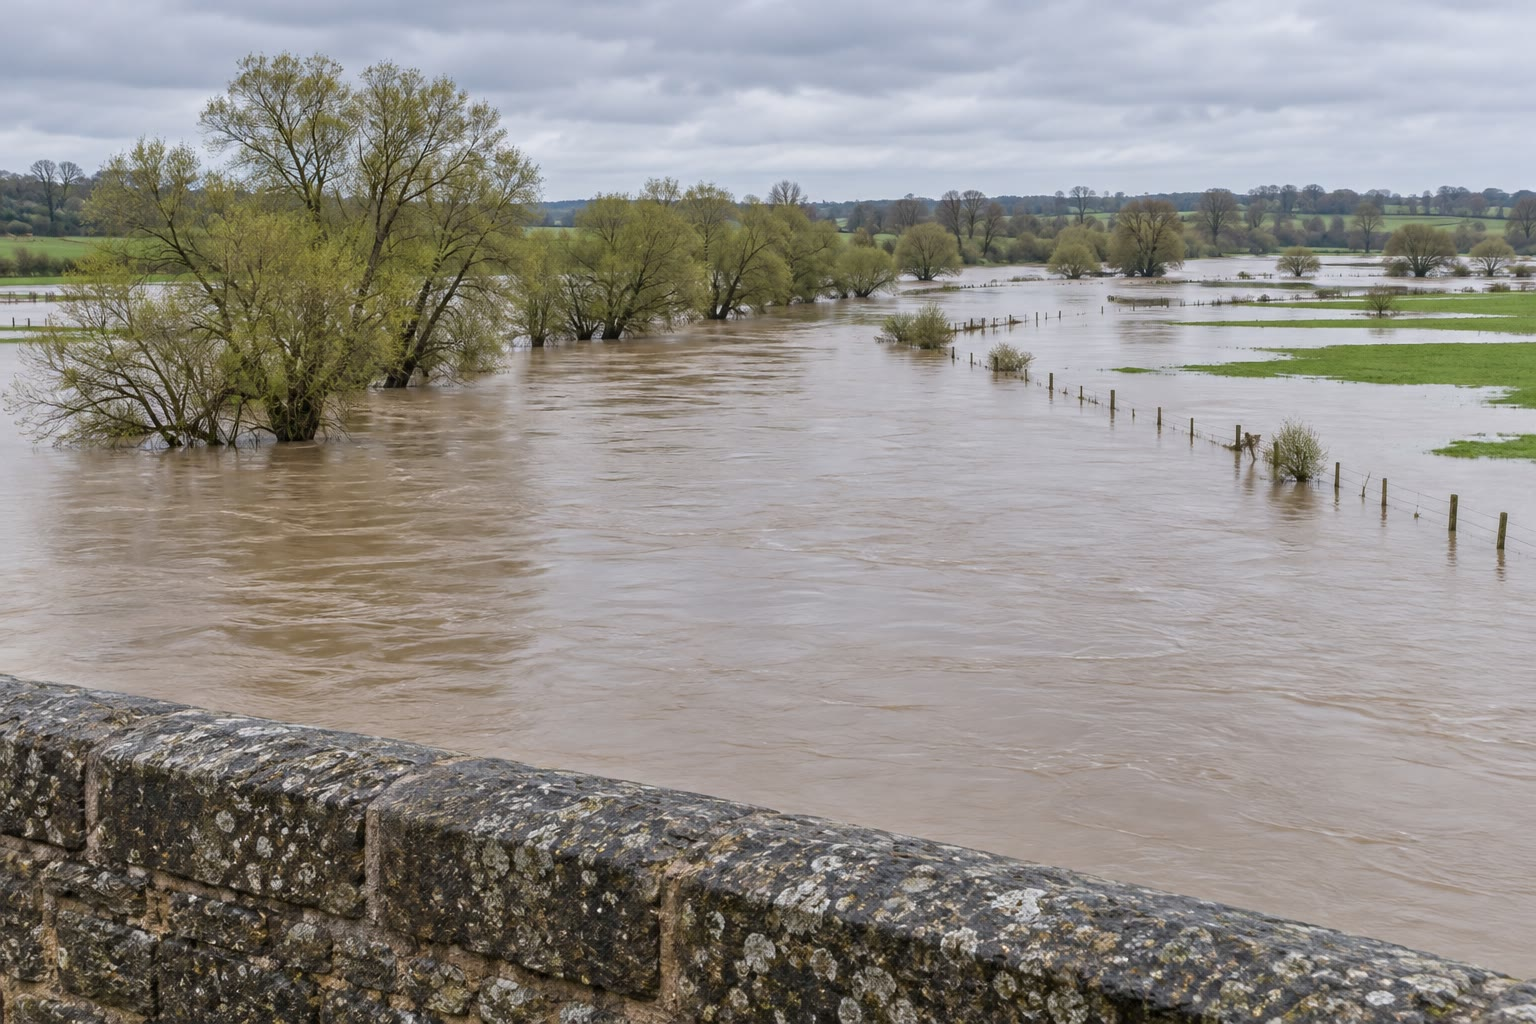
\includegraphics[width=0.8\linewidth]{images/book2/ai/g10-river-flood-meadows.jpg}

{\small Un río en crecida visto desde un puente de piedra: el agua parda,
cargada de barro, ha salido de su cauce y cubre los prados de su llanura de
inundación, hasta las cercas y los árboles que bordean sus orillas
habituales.}
\end{omfigure}

\begin{recall}
La lluvia que llega al suelo se infiltra en él, corre por su superficie o se
evapora; el ciclo del agua la devuelve al mar (los libros de física). El agua se infiltra en las rocas permeables y las llena por debajo
del nivel freático, formando acuíferos que alimentan manantiales y ríos
(Libro 1, año 6). Un río serpentea en meandros por su llanura de inundación,
plana, que cubre cuando crece (Libro 1, año 5). Las curvas de nivel unen
puntos de igual altura; las Colinas de Varden son la región dibujada en los
mapas de esta serie (Libro 1, años 2 y 9).
\end{recall}

\begin{safety}
El agua de una crecida es mucho más peligrosa de lo que parece. Unos
\qty{15}{cm} de agua que corre deprisa pueden derribar a un adulto, y unos
\qty{30}{cm} pueden arrastrar un coche; puede que la carretera de debajo se
haya hundido. No entres nunca a pie ni en coche en el agua de una crecida:
da la vuelta y ve por otro camino.
% ledger: nws:flood-water
\end{safety}

\section{La cuenca hidrográfica}

Cada gota de lluvia que no se evapora ni se infiltra en profundidad corre
cuesta abajo. Sigue la mayor pendiente del terreno, se une a un reguero,
después a un arroyo, y los arroyos se juntan en ríos. Toda la tierra cuya
agua acaba en un mismo río forma una unidad.

\begin{definition}[Cuenca hidrográfica; divisoria de aguas]\label{def:g10:drainage-basins:drainage-basin}
La \emph{cuenca hidrográfica}\index{cuenca hidrografica@cuenca hidrográfica}
de un punto de un río es toda la superficie de tierra cuya escorrentía va a
parar al río aguas arriba de ese punto y pasa por él. La
\emph{divisoria de aguas}\index{divisoria de aguas} es la línea que separa dos cuencas hidrográficas vecinas:
sigue las crestas del terreno, y la lluvia que cae a uno y otro lado de ella
va a parar a ríos distintos.
\end{definition}

Una cuenca se define siempre para un punto del río, su \emph{punto de
salida}: la cuenca de un río donde llega al mar es la mayor, y cada punto
aguas arriba tiene dentro una cuenca más pequeña. Dos gotas que caen a un
metro una de otra, a ambos lados de una divisoria, pueden acabar en ríos
distintos e incluso en océanos distintos.

\subsection*{La cuenca del río Varden}

Un ordenador encuentra una \omterm{def:g10:drainage-basins:drainage-basin}{cuenca hidrográfica} a partir de un mapa de alturas
en unos pocos pasos. El mapa se divide en pequeños cuadrados, aquí de
\qty{50}{m} de lado. Para cada cuadrado, el ordenador mira sus ocho vecinos y
envía el agua al que alcanza por la pendiente descendente más fuerte. (Donde
una pequeña hondonada no tiene ningún vecino más bajo, primero se llena hasta
el nivel al que desbordaría, como hace un charco.) Siguiendo estos pasos de
cuadrado en cuadrado se traza el camino de una gota desde cualquier punto del
mapa. Los cuadrados cuyas gotas llegan al río forman la cuenca.

\begin{omfigure}
\begin{tikzpicture}
\begin{axis}[axis equal image, xmin=0, xmax=10, ymin=0, ymax=8, width=0.86\linewidth,
  tick label style={font=\scriptsize}, xlabel={este (km)}, ylabel={norte (km)},
  label style={font=\small}, enlargelimits=false]
\addplot[fill=omDef!14, draw=none, even odd rule] table {figdata/out/grade-10-varden_basin-fill.dat};
\addplot[contour, line width=0.25pt, opacity=0.7] table {figdata/out/shared-region-contours.dat};
\addplot[index contour, opacity=0.8] table {figdata/out/shared-region-index-contours.dat};
\addplot[river, line width=1.6pt] table {figdata/out/shared-region-river.dat};
\addplot[omThm, line width=1.4pt, dashed] table {figdata/out/grade-10-varden_basin-divide.dat};
\addplot[omWxRain, line width=0.9pt, -{Stealth[length=5pt]}] table {figdata/out/grade-10-varden_basin-path1.dat};
\addplot[omWxRain, line width=0.9pt, -{Stealth[length=5pt]}] table {figdata/out/grade-10-varden_basin-path2.dat};
\addplot[omWxRain, line width=0.9pt, -{Stealth[length=5pt]}] table {figdata/out/grade-10-varden_basin-path3.dat};
\addplot[omWxRain, line width=0.9pt, -{Stealth[length=5pt]}] table {figdata/out/grade-10-varden_basin-path4.dat};
\fill[omWxRain] (axis cs:2,7.4) circle (2.2pt);
\fill[omWxRain] (axis cs:4,1.8) circle (2.2pt);
\fill[omWxRain] (axis cs:8.6,6.6) circle (2.2pt);
\fill[omWxRain] (axis cs:2.5,0.7) circle (2.2pt);
\node[font=\footnotesize, fill=white, fill opacity=0.85, text opacity=1, inner sep=1.5pt, text=omThm] at (axis cs:6.0,6.75) {divisoria};
\node[font=\footnotesize, fill=white, fill opacity=0.85, text opacity=1, inner sep=1.5pt, text=omThm] at (axis cs:3.5,1.1) {divisoria};
\node[font=\footnotesize, fill=white, fill opacity=0.85, text opacity=1, inner sep=1.5pt, align=center] at (axis cs:5.3,7.55) {fuera de la cuenca:\\el agua sale hacia el norte};
\node[font=\footnotesize, fill=white, fill opacity=0.85, text opacity=1, inner sep=1.5pt, align=right, anchor=east] at (axis cs:9.85,3.35) {punto de\\salida};
\draw[-{Stealth[length=6pt]}, line width=1pt, omRiver] (axis cs:9.3,3.7) -- (axis cs:9.95,4.15);
\node[font=\footnotesize, fill=white, fill opacity=0.85, text opacity=1, inner sep=1.5pt] at (axis cs:1.1,4.75) {río};
\end{axis}
\end{tikzpicture}

{\small La \omterm{def:g10:drainage-basins:drainage-basin}{cuenca hidrográfica} del río Varden en el mapa de las Colinas de
Varden (sombreada), calculada enviando el agua de cada cuadrado de
\qty{50}{m} por la mayor pendiente; curvas de nivel cada \qty{50}{m}. Las
líneas discontinuas son las divisorias; las líneas azules son los caminos de
cuatro gotas de lluvia (puntos). Dos llegan al río y fluyen hacia el este
hasta el punto de salida, donde el río sale del mapa; las otras dos, más allá
de las divisorias, salen del mapa hacia otros ríos.}
\end{omfigure}

La cuenca cubre \qty{66}{km^2} de los \qty{80}{km^2} del mapa, unas cuatro
quintas partes. En el norte, la divisoria sigue las crestas de las
colinas y pasa por sus cumbres; más allá, el terreno desciende en sentido contrario al río y su
agua va a otro valle. En la esquina suroeste, una pequeña zona también
desagua fuera del mapa. El propio río entra en el mapa por el oeste, así que
su cuenca completa es mayor: abarca también las tierras de aguas arriba, más
allá del borde del mapa.
% values computed in figdata/grade-10/varden_basin.py (basin_km2 66.19, map_km2 80)

\subsection*{Los ríos más grandes}

Los ríos se comparan por la superficie de su cuenca y por el agua que llevan.
El río más grande del mundo, con mucha diferencia, es el Amazonas. El
Misisipi, el río más grande de Estados Unidos, drena unas \num{1150000}
millas cuadradas, unos 2.98 millones de \unit{km^2}, de Estados Unidos y
Canadá.
% ledger: kammerer:mississippi

\section{El caudal}

\begin{definition}[Caudal]\label{def:g10:drainage-basins:discharge}
El \emph{caudal}\index{caudal} de un río en un punto es el volumen de agua
que atraviesa una sección transversal del río en un segundo. Se mide en
metros cúbicos por segundo, \unit{m^3/s}.
\end{definition}

Un \omterm{def:g10:drainage-basins:discharge}{caudal} de \qty{1}{m^3/s} son mil litros cada segundo, o
\qty{86400}{m^3} al día. El agua corre más deprisa cerca de la superficie, en
el centro del cauce, y más despacio a lo largo del lecho y de las orillas,
donde roza con ellos; la \emph{velocidad media} es la velocidad promediada
sobre toda la sección transversal.

\begin{proposition}[Caudal, velocidad y sección transversal]\label{prop:g10:drainage-basins:discharge}
El \omterm{def:g10:drainage-basins:discharge}{caudal} $Q$ de un río es el producto de la velocidad media $v$ del agua por
el área $A$ de la sección mojada:
\[
Q = v\,A.
\]
\end{proposition}

\begin{proof}
En un tiempo $t$, el agua que atraviesa la sección ha avanzado una
distancia $v\,t$: llena un tramo del río de sección $A$ y
longitud $v\,t$, de volumen $A\,v\,t$. Dividiendo este volumen entre el tiempo $t$
se obtiene el volumen por segundo, $Q = v\,A$.
\end{proof}

Un río con una sección transversal de \qty{50}{m^2} que corre a una velocidad
media de \qty{1.2}{m/s} lleva $1.2 \times 50 = \qty{60}{m^3/s}$. En crecida,
los dos factores aumentan: el agua gana profundidad y anchura, así que la
sección crece, y corre más deprisa.

\subsection*{Medir un caudal}

Como la velocidad cambia de una orilla a otra, se mide en varios puntos. El
río se divide en franjas verticales; en cada una se miden la profundidad y la
velocidad, y se suman los \omterm{def:g10:drainage-basins:discharge}{caudales} de las franjas.

\begin{method}[El método velocidad--área]\label{met:g10:drainage-basins:velocity-area}
\begin{enumerate}
  \item Tiende una cinta métrica de una orilla a otra y elige verticales a
        intervalos regulares $w$ a lo largo de ella.
  \item En cada vertical, mide con un molinete la profundidad $d$ y la
        velocidad media $v$ del agua en esa profundidad.
  \item Cada vertical representa una franja de anchura $w$ y área $w\,d$; su
        \omterm{def:g10:drainage-basins:discharge}{caudal} es $v\,w\,d$.
  \item Suma los \omterm{def:g10:drainage-basins:discharge}{caudales} de todas las franjas: $Q = \sum v\,w\,d$.
        La sección transversal es $A = \sum w\,d$, y la velocidad media, $Q/A$.
\end{enumerate}
\end{method}

\begin{omfigure}
\begin{tikzpicture}[x=0.9cm, y=1.6cm, font=\footnotesize]
  % water
  \fill[omSea] (0,0) -- (1,-0.4) -- (2,-0.75) -- (3,-1.0) -- (4,-1.25) -- (5,-1.4) -- (6,-1.3)
     -- (7,-1.1) -- (8,-0.8) -- (9,-0.5) -- (10,-0.2) -- (10.5,0) -- cycle;
  \fill[omDef!22] (4,0) -- (4,-1.25) -- (5,-1.4) -- (6,-1.3) -- (6,0) -- cycle;
  % bed
  \draw[line width=0.9pt, brown!60!black] (-0.6,0.35) -- (0,0) -- (1,-0.4) -- (2,-0.75) -- (3,-1.0) -- (4,-1.25)
     -- (5,-1.4) -- (6,-1.3) -- (7,-1.1) -- (8,-0.8) -- (9,-0.5) -- (10,-0.2) -- (10.5,0) -- (11.1,0.35);
  \draw[omDef!70!black, line width=0.5pt] (0,0) -- (10.5,0);
  % verticals
  \foreach \x/\d/\v/\dx in {1/0.4/0.3/0.3, 3/1.0/0.6/0, 5/1.4/0.8/0, 7/1.1/0.7/0, 9/0.5/0.4/-0.25} {
    \draw[black!70, dashed] (\x,0) -- (\x,-\d);
    \node[anchor=south, font=\scriptsize] at (\x,0.02) {\qty{\v}{m/s}};
    \node[font=\scriptsize, fill=white, inner sep=0.8pt] at (\x+\dx,-0.5*\d) {\qty{\d}{m}};
  }
  \draw[{Stealth}-{Stealth}] (4,0.42) -- node[above, font=\scriptsize] {una franja: $w = \qty{2}{m}$} (6,0.42);
  \node[anchor=west, align=left] at (11.2,-0.15) {superficie\\del agua};
  \node[anchor=west, align=left] at (11.2,-0.9) {lecho};
  \draw[black!50] (11.15,-0.9) -- (8.5,-0.68);
  \node[anchor=north] at (5.25,-1.75) {velocidades medias medidas en las verticales (sobre el agua) y profundidades (en el agua)};
\end{tikzpicture}

{\small Medida de un \omterm{def:g10:drainage-basins:discharge}{caudal} (esquema; escala vertical exagerada). Cinco
verticales, separadas \qty{2}{m}, dividen en franjas un arroyo de unos
\qty{10}{m} de ancho; la franja sombreada es la medida en la vertical central.}
\end{omfigure}

\begin{example}[Un aforo]\label{ex:g10:drainage-basins:gauging}
En el arroyo de la figura, las cinco franjas, de \qty{2}{m} de ancho cada una,
tienen áreas de $2 \times 0.4 = 0.8$, $2.0$, $2.8$, $2.2$ y \qty{1.0}{m^2}: la
sección transversal es de \qty{8.8}{m^2}. Sus \omterm{def:g10:drainage-basins:discharge}{caudales} son $0.3 \times 0.8 =
0.24$, $0.6 \times 2.0 = 1.20$, $0.8 \times 2.8 = 2.24$, $0.7 \times 2.2 =
1.54$ y $0.4 \times 1.0 = \qty{0.40}{m^3/s}$, así que el arroyo lleva
$Q \approx \qty{5.6}{m^3/s}$. La velocidad media es de $5.62/8.8 \approx
\qty{0.64}{m/s}$, menos que los \qty{0.8}{m/s} del centro del arroyo.
\end{example}

\begin{omfigure}
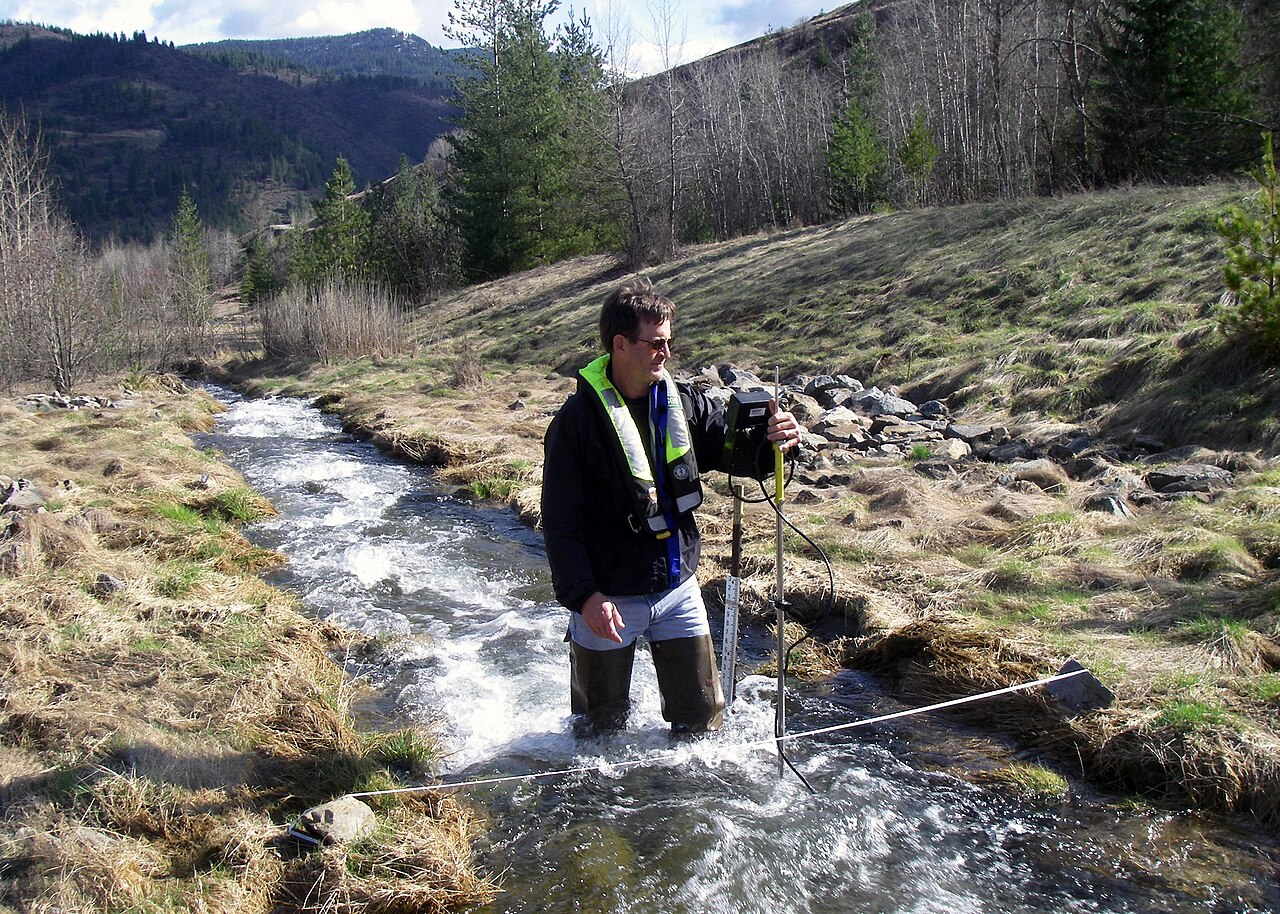
\includegraphics[height=4.6cm]{images/book2/g10-usgs-hydrologist-streamflow.jpg}\hspace{0.3cm}%
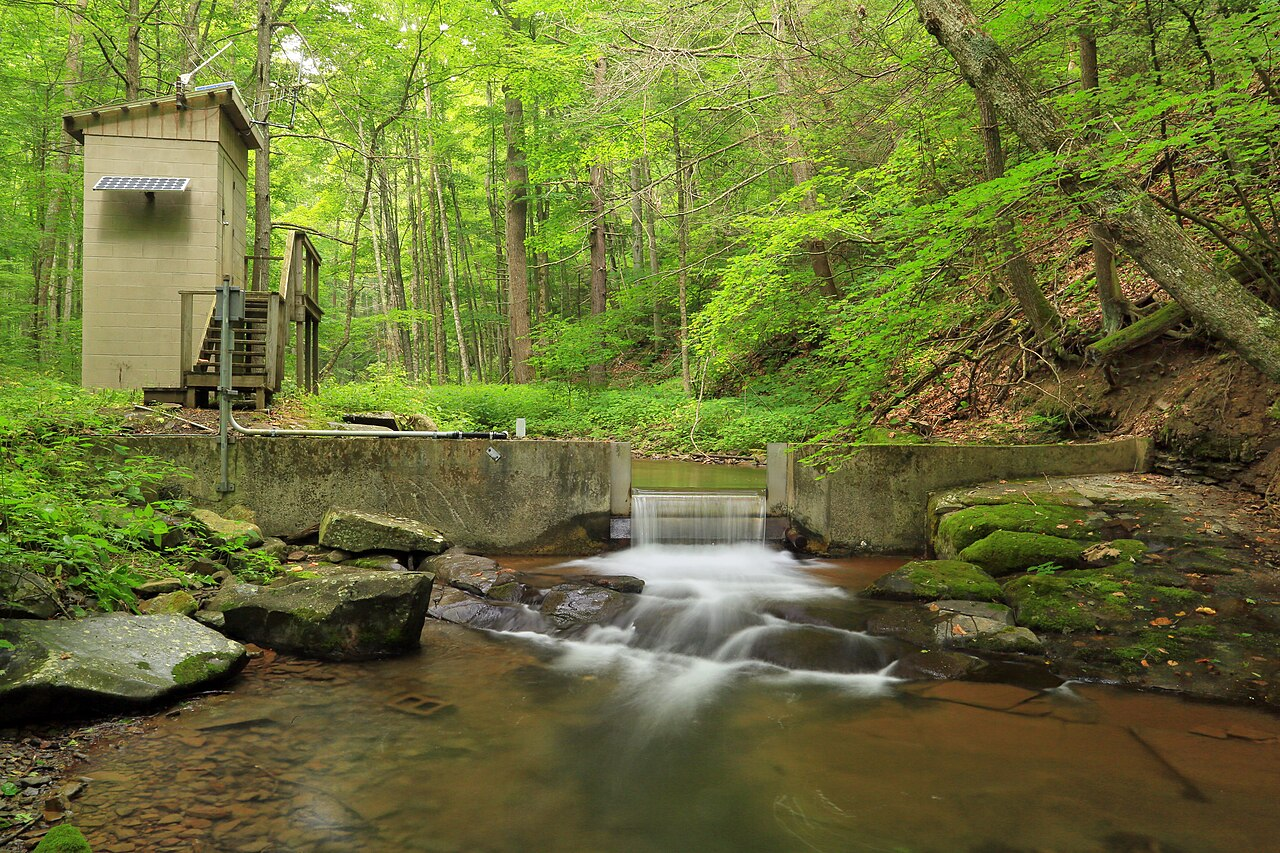
\includegraphics[height=4.6cm]{images/book2/g10-usgs-streamgage.jpg}

{\small Izquierda: una hidróloga mide el \omterm{def:g10:drainage-basins:discharge}{caudal} de un arroyo de montaña por
el método velocidad--área; la cinta tendida de una orilla a otra marca las
verticales, y la pértiga lleva un molinete. Derecha: una estación de aforo en
un arroyo de bosque; la caseta guarda los instrumentos que registran el nivel
del agua detrás del pequeño vertedero. Fotografías: U.S. Geological Survey
(dominio público).}
\end{omfigure}

Un aforo lleva tiempo y no puede hacerse de forma continua. Una estación de
aforo registra, en cambio, el nivel del agua, sin interrupción. Unos pocos
aforos hechos a niveles distintos dan una curva que relaciona el nivel con el
\omterm{def:g10:drainage-basins:discharge}{caudal}, y la estación convierte en \omterm{def:g10:drainage-basins:discharge}{caudal} cada nivel que registra.

Los grandes ríos llevan \omterm{def:g10:drainage-basins:discharge}{caudales} enormes. De 1972 a 2003, el Amazonas
vertió al océano Atlántico una media de unos \qty{206000}{m^3/s}, con un
margen de un \qty{6}{\percent}: alrededor del \qty{17}{\percent} de toda el
agua dulce que los ríos del mundo llevan al mar. El Misisipi lleva al golfo de
México una media de \num{593000} pies cúbicos por segundo, unos
\qty{16800}{m^3/s}: el Amazonas lleva unas doce veces más.
% ledger: callede:amazon, kammerer:mississippi

\section{El hidrograma}

\begin{definition}[Hidrograma; caudal base; tiempo de retardo]\label{def:g10:drainage-basins:hydrograph}
Un \emph{hidrograma}\index{hidrograma} es la gráfica del \omterm{def:g10:drainage-basins:discharge}{caudal} de un río en
un punto en función del tiempo. El \emph{caudal base}\index{caudal base} es
la parte del \omterm{def:g10:drainage-basins:discharge}{caudal} alimentada por el agua subterránea, que mantiene el río
en marcha entre lluvias. El \emph{tiempo de retardo}\index{tiempo de retardo}
de una crecida es el tiempo que pasa entre el máximo de la lluvia sobre la
cuenca y el pico del \omterm{def:g10:drainage-basins:discharge}{caudal}.
\end{definition}

\begin{omfigure}
\begin{tikzpicture}[x=1cm, y=1cm, font=\footnotesize]
  \draw[-{Stealth}] (0,0) -- (10.2,0) node[below left] {tiempo};
  \draw[-{Stealth}] (0,0) -- (0,5.9) node[above right] {caudal};
  % rain bars hanging from the top
  \draw[black!50] (0,5.4) -- (10,5.4);
  \foreach \x/\h in {1.0/0.15, 1.3/0.35, 1.6/0.55, 1.9/0.4, 2.2/0.2} {
    \fill[omWxRain!70] (\x,5.4) rectangle ++(0.28,-\h);
  }
  \node[anchor=south west] at (2.6,5.4) {lluvia sobre la cuenca};
  % baseflow and hydrograph
  \fill[omSea] (0,0.7) -- (2.0,0.7) .. controls (2.8,0.8) and (3.3,3.3) .. (4.0,3.6)
    .. controls (4.6,3.6) and (5.1,2.1) .. (6.0,1.55) .. controls (7.0,1.0) and (8.0,0.85) .. (10,0.8)
    -- (10,0) -- (0,0) -- cycle;
  \fill[omLithAlluv] (0,0) -- (0,0.7) -- (2.0,0.7) .. controls (3.5,0.68) and (5.5,0.75) .. (6.6,0.95)
    .. controls (8,1.0) and (9,0.85) .. (10,0.8) -- (10,0) -- cycle;
  \draw[omDef, line width=1.2pt] (0,0.7) -- (2.0,0.7) .. controls (2.8,0.8) and (3.3,3.3) .. (4.0,3.6)
    .. controls (4.6,3.6) and (5.1,2.1) .. (6.0,1.55) .. controls (7.0,1.0) and (8.0,0.85) .. (10,0.8);
  \draw[black!60, dashed] (2.0,0.7) .. controls (3.5,0.68) and (5.5,0.75) .. (6.6,0.95);
  % lag time
  \draw[black!60, densely dotted] (1.74,4.85) -- (1.74,4.3);
  \draw[black!60, densely dotted] (3.98,3.65) -- (3.98,4.3);
  \draw[{Stealth}-{Stealth}] (1.74,4.3) -- node[above] {tiempo de retardo} (3.98,4.3);
  % labels
  \node[anchor=west] at (4.2,3.75) {pico};
  \node[anchor=east, align=right] at (2.9,2.2) {rama\\ascendente};
  \node[anchor=west, align=left] at (5.4,2.3) {rama descendente};
  \node[align=center] at (4.5,1.25) {escorrentía};
  \node at (8.2,0.4) {caudal base};
\end{tikzpicture}

{\small El \omterm{def:g10:drainage-basins:hydrograph}{hidrograma} de una crecida (esquema). Después de la lluvia, el
\omterm{def:g10:drainage-basins:discharge}{caudal} sube hasta un pico y vuelve a bajar más despacio; el área bajo la
curva es el volumen de agua. El \omterm{def:g10:drainage-basins:hydrograph}{caudal base}, alimentado por el agua
subterránea, cambia poco; el resto es la escorrentía que la lluvia mandó
rápidamente al río.}
\end{omfigure}

El agua de una tormenta llega al río en momentos distintos. La lluvia que cae
cerca del cauce llega en minutos u horas; la que cae muy aguas arriba tarda
mucho más, porque tiene que bajar por las laderas y a lo largo del río. Por
eso el \omterm{def:g10:drainage-basins:discharge}{caudal} sube bruscamente, en la \emph{rama ascendente}, mientras llega
el agua de las laderas cercanas; alcanza su pico cuando llega más agua a la
vez, y baja más despacio, en la \emph{rama descendente}, a medida que se
escurre la última agua de los rincones lejanos de la cuenca y del suelo.
Cuanto mayor es la cuenca, más largo es el \omterm{def:g10:drainage-basins:hydrograph}{tiempo de retardo}: horas para un
arroyo pequeño, días para un gran río.

Algunas cuencas dan crecidas \emph{súbitas}, con un pico alto y repentino y
un \omterm{def:g10:drainage-basins:hydrograph}{tiempo de retardo} corto; otras dan crecidas lentas y aplanadas. La misma
lluvia da una crecida más súbita cuando:
\begin{itemize}
  \item la cuenca es pequeña y empinada, de modo que el agua tiene un camino
        corto y rápido;
  \item el suelo deja infiltrarse poca agua: roca desnuda, arcilla, suelo ya
        empapado, suelo helado y, sobre todo, los tejados, las calles y los
        aparcamientos de una ciudad, que mandan casi toda la lluvia
        directamente a los desagües y a los arroyos;
  \item la cuenca tiene una red densa de arroyos y desagües, que recoge el
        agua deprisa.
\end{itemize}
Los bosques, los suelos profundos y permeables y las llanuras de inundación
anchas hacen lo contrario: retienen el agua y la sueltan despacio, lo que
rebaja y retrasa el pico.

\subsection*{Una crecida real}

El río Potomac drena una cuenca de \num{11560} millas cuadradas, unos
\qty{29900}{km^2}, aguas arriba de una estación de aforo cercana a
Washington, en el este de Estados Unidos. En enero de 1996 la estación
registró el \omterm{def:g10:drainage-basins:hydrograph}{hidrograma} siguiente.
% ledger: data:b2-usgs-potomac

\begin{omfigure}
\begin{tikzpicture}
\begin{axis}[omrecord, width=0.86\linewidth, height=6cm, xmin=0, xmax=55, ymin=0, ymax=10000,
  xtick={0,10,20,30,40,50}, xticklabels={5 ene, 15 ene, 25 ene, 4 feb, 14 feb, 24 feb},
  ylabel={caudal (\unit{m^3/s})}, xlabel={1996},
  tick label style={font=\small}, label style={font=\small},
  scaled y ticks=false, yticklabel style={/pgf/number format/fixed}]
\addplot[omDef, line width=1.1pt, mark=*, mark size=1.1pt] table[x=day, y=q] {figdata/out/grade-10-flood_frequency-hydrograph.dat};
\node[anchor=west, font=\footnotesize] at (axis cs:17,9231) {\qty{9231}{m^3/s} el 21 de enero};
\draw[black!60, dashed] (axis cs:5,334) -- (axis cs:13,334);
\node[anchor=south, font=\footnotesize] at (axis cs:9,1000) {unos \qty{330}{m^3/s}};
\draw[black!60] (axis cs:9,1000) -- (axis cs:9,390);
\end{axis}
\end{tikzpicture}

{\small \omterm{def:g10:drainage-basins:discharge}{Caudal} medio diario del río Potomac cerca de Washington del 5 de enero
al 29 de febrero de 1996: la crecida subió de \qty{362}{m^3/s} el 18 de enero
a más de \qty{9000}{m^3/s} tres días después, y luego bajó a lo largo de las
semanas siguientes, con una segunda subida más pequeña a finales de enero.
Datos: U.S. Geological Survey, estación 01646500.}
\end{omfigure}
% values computed in figdata/grade-10/flood_frequency.py (hydro_peak_m3s 9231, hydro_before_mean 334)

En los días anteriores a la crecida, el río llevaba unos \qty{330}{m^3/s}, su
\omterm{def:g10:drainage-basins:hydrograph}{caudal base}. El 21 de enero la media diaria alcanzó \qty{9231}{m^3/s}, casi
treinta veces más. Repartida sobre toda la cuenca, el agua que pasó ese día
por la estación formaría una capa de
$9231 \times 86400 / (29\,900 \times 10^6) \approx \qty{0.027}{m}$, unos
\qty{27}{mm} de espesor: una lluvia fuerte, entregada en un solo día por toda
la cuenca a la vez.
% ledger: data:b2-usgs-potomac (hydro_peak_mm_per_day 26.6 in figdata/grade-10/flood_frequency.py)

\section{Las crecidas y su periodo de retorno}

¿Qué tamaño de crecida debe esperar una ciudad? La respuesta viene del
pasado: una estación de aforo que funciona desde hace décadas ha registrado
el mayor \omterm{def:g10:drainage-basins:discharge}{caudal} de cada año, el \emph{pico anual}. Los picos pequeños llegan
casi todos los años; los grandes, rara vez. Cuanto más rara es una crecida,
mayor es.

\begin{definition}[Periodo de retorno]\label{def:g10:drainage-basins:return-period}
El \emph{periodo de retorno}\index{periodo de retorno} $T$ de una crecida es
el intervalo medio, en años, entre los años cuyo pico anual la iguala o la
supera. Una crecida de periodo de retorno $T$, una \emph{crecida de $T$ años},
tiene una probabilidad $1/T$ de ser igualada o superada en un año cualquiera.
\end{definition}

Una crecida de cien años no es una crecida que llega una vez cada cien años,
como un horario. Es una crecida que tiene una probabilidad entre cien de ser
igualada o superada cada año, todos los años, pase lo que pase el año
anterior. Pueden llegar dos en años seguidos; puede pasar un siglo sin
ninguna.

\begin{method}[Periodos de retorno a partir de un registro de picos anuales]\label{met:g10:drainage-basins:return-periods}
\begin{enumerate}
  \item Haz la lista de los picos anuales de $n$ años.
  \item Ordénalos del mayor (rango $m = 1$) al menor
        (rango $m = n$).
  \item Asigna al pico de rango $m$ el \omterm{def:g10:drainage-basins:return-period}{periodo de retorno} $T = (n + 1)/m$.
  \item Representa los picos frente a $T$ en una escala logarítmica de $T$,
        y lee el \omterm{def:g10:drainage-basins:discharge}{caudal} correspondiente al \omterm{def:g10:drainage-basins:return-period}{periodo de retorno} buscado.
\end{enumerate}
\end{method}

Así, el mayor de $n$ picos recibe $T = n + 1$ años: en un registro de
\num{95} años, \num{96} años. La fórmula refleja lo que muestra el registro:
el pico de rango $m$ ha sido igualado o superado en $m$ de los $n$ años, más
o menos una vez cada $n/m$ años. El método no puede ir con fiabilidad más
allá de la longitud del registro: un registro de \num{50} años dice poco
sobre la crecida de \num{1000} años.

\begin{omfigure}
\begin{tikzpicture}
\begin{axis}[omrecord, width=0.86\linewidth, height=6.2cm, xmode=log, xmin=0.9, xmax=150,
  ymin=0, ymax=15000, xlabel={periodo de retorno $T$ (años)}, ylabel={pico anual (\unit{m^3/s})},
  xtick={1,2,5,10,20,50,100}, xticklabels={1,2,5,10,20,50,100},
  tick label style={font=\small}, label style={font=\small},
  scaled y ticks=false, yticklabel style={/pgf/number format/fixed}]
\addplot[only marks, mark=*, mark size=1.5pt, omDef] table[x=T, y=peak] {figdata/out/grade-10-flood_frequency-ranked.dat};
\node[anchor=east, font=\footnotesize] at (axis cs:92,13705) {1936};
\node[anchor=east, font=\footnotesize] at (axis cs:46,12658) {1942};
\node[anchor=south, font=\footnotesize] at (axis cs:32,10300) {1972};
\node[anchor=north west, font=\footnotesize, align=left] at (axis cs:1.1,14000) {río Potomac cerca de Washington,\\picos anuales 1931--2025 ($n = 95$)};
\end{axis}
\end{tikzpicture}

{\small Los \num{95} picos anuales del río Potomac cerca de Washington,
ordenados y representados frente a sus \omterm{def:g10:drainage-basins:return-period}{periodos de retorno} $T = (n+1)/m$. El
mayor, en marzo de 1936, recibe $T = 96$ años. Datos: U.S. Geological Survey,
estación 01646500.}
\end{omfigure}
% values computed in figdata/grade-10/flood_frequency.py

\begin{dated}{2026}
En el registro del Potomac cerca de Washington, de 1931 a 2025, los cinco
mayores picos anuales se produjeron en marzo de 1936 (\qty{13700}{m^3/s}),
octubre de 1942, junio de 1972, abril de 1937 y enero de 1996, estos dos
últimos iguales, con \qty{9830}{m^3/s}.
% ledger: data:b2-usgs-potomac
\end{dated}

\subsection*{La probabilidad de una crecida a lo largo de muchos años}

Una casa o un puente duran décadas. Lo que les importa no es la probabilidad
de una crecida en un año, sino a lo largo de toda su vida.

\begin{proposition}[Al menos una crecida en $N$ años]\label{prop:g10:drainage-basins:chance}
Si los años son independientes entre sí, la probabilidad de que una crecida
de \omterm{def:g10:drainage-basins:return-period}{periodo de retorno} $T$ sea igualada o superada al menos una vez en $N$
años es
\[
P = 1 - \left(1 - \frac{1}{T}\right)^{N}.
\]
\end{proposition}

\begin{proof}
En un año, la probabilidad de que la crecida \emph{no} ocurra es
$1 - 1/T$. Como los años son independientes, la probabilidad de que no ocurra
en ninguno de los $N$ años es el producto de $N$ factores así, $(1 - 1/T)^N$.
El suceso ``al menos una vez'' es el contrario de ``nunca'', así que su
probabilidad es $1 - (1 - 1/T)^N$.
\end{proof}

Para una crecida de cien años a lo largo de treinta años, $(0.99)^{30} \approx 0.740$, y $P \approx 0.26$: una probabilidad de una entre cuatro. A
lo largo de cien años, $(0.99)^{100}
\approx 0.366$ y $P \approx 0.63$: está lejos de ser seguro que la crecida de
cien años llegue en cien años.

\begin{omfigure}
\begin{tikzpicture}
\begin{axis}[omrecord, width=0.82\linewidth, height=5.8cm, xmin=0, xmax=100, ymin=0, ymax=1,
  xlabel={número de años $N$}, ylabel={probabilidad de al menos una crecida},
  ytick={0,0.2,0.4,0.6,0.8,1}, yticklabels={0, 20\,\%, 40\,\%, 60\,\%, 80\,\%, 100\,\%},
  tick label style={font=\small}, label style={font=\small},
  legend pos=south east, legend style={font=\footnotesize}]
\addplot[omThm, line width=1pt] table[x=n, y=p10] {figdata/out/grade-10-flood_frequency-chance.dat};
\addplot[omProp, line width=1pt] table[x=n, y=p50] {figdata/out/grade-10-flood_frequency-chance.dat};
\addplot[omDef, line width=1pt] table[x=n, y=p100] {figdata/out/grade-10-flood_frequency-chance.dat};
\legend{{crecida de 10 años}, {crecida de 50 años}, {crecida de 100 años}}
\draw[black!60, dashed] (axis cs:30,0) -- (axis cs:30,0.2603) -- (axis cs:0,0.2603);
\fill[omDef] (axis cs:30,0.2603) circle (2pt);
\node[anchor=north west, font=\footnotesize] at (axis cs:31,0.22) {26\,\% en 30 años};
\end{axis}
\end{tikzpicture}

{\small La probabilidad de que una crecida de \omterm{def:g10:drainage-basins:return-period}{periodo de retorno} 10, 50 o
100 años llegue al menos una vez en $N$ años.}
\end{omfigure}
% values computed in figdata/grade-10/flood_frequency.py (chance_100_30 0.2603)

\section{Presas y diques}

Hace mucho que construimos estructuras que cambian el paso de una crecida.
Dos de ellas lo cambian en sentidos opuestos.

Una \emph{presa} retiene un embalse. Cuando llega una crecida, parte de su
agua se almacena en el embalse, cuyo nivel sube, y se suelta después, a lo
largo de más tiempo. Aguas abajo pasa el mismo volumen de agua, pero
repartido: el pico es más bajo y más tardío. Un embalse solo rebaja una
crecida mientras le queda sitio; una vez lleno, toda el agua que entra sigue
su camino.

Un \emph{dique} es un terraplén de tierra construido a lo largo de un río
para mantener sus crecidas fuera de la llanura de inundación. Entre los
diques, el agua no puede extenderse; para llevar el mismo \omterm{def:g10:drainage-basins:discharge}{caudal} por una
sección más estrecha, tiene que subir más y correr más deprisa. Las tierras de
detrás de los diques siguen secas, mientras los diques aguanten y el agua no
los rebase. Pero la llanura de inundación ya no almacena agua durante la
crecida, así que una mayor parte de ella baja, y antes, aguas abajo.

\begin{omfigure}
\begin{tikzpicture}[x=0.62cm, y=0.62cm, font=\footnotesize]
  \begin{scope}
    \draw[-{Stealth}] (0,0) -- (9.4,0) node[below left] {tiempo};
    \draw[-{Stealth}] (0,0) -- (0,6.0) node[above right] {caudal};
    \draw[omDef, line width=1.2pt] (0,0.6) -- (1,0.6) .. controls (1.8,0.7) and (2.2,5.2) .. (2.8,5.2)
      .. controls (3.5,5.2) and (4,1.6) .. (5,1.0) .. controls (6,0.7) and (7.5,0.6) .. (9,0.6);
    \draw[omThm, line width=1.2pt, dashed] (0,0.6) -- (1.3,0.6) .. controls (2.3,0.75) and (3.0,3.3) .. (3.8,3.3)
      .. controls (4.7,3.3) and (5.8,1.5) .. (6.8,1.0) .. controls (7.6,0.75) and (8.3,0.65) .. (9,0.6);
    \node[anchor=west, text=omDef] at (3.0,5.35) {entrada al embalse};
    \node[anchor=west, text=omThm] at (4.2,3.55) {bajo la presa};
    \node[anchor=north] at (4.5,-0.45) {(a) una presa: pico más bajo y tardío};
  \end{scope}
  \begin{scope}[xshift=7.2cm]
    \fill[omLithAlluv] (0,0) -- (10,0) -- (10,1.8) -- (0,1.8) -- cycle;
    \fill[white] (3.5,1.8) -- (3.9,0.4) -- (6.1,0.4) -- (6.5,1.8) -- cycle;
    \fill[omSea] (0.4,2.3) -- (3.25,2.3) -- (3.5,1.8) -- (3.9,0.4) -- (6.1,0.4) -- (6.5,1.8) -- (6.75,2.3) -- (9.6,2.3) -- (9.6,1.8) -- (0.4,1.8) -- cycle;
    \draw[line width=0.8pt, brown!60!black] (0,1.8) -- (3.5,1.8) -- (3.9,0.4) -- (6.1,0.4) -- (6.5,1.8) -- (10,1.8);
    \draw[omDef!70!black] (0.4,2.3) -- (9.6,2.3);
    \node[anchor=south, text=omDef!70!black, align=center] at (1.5,2.35) {sin\\diques};
    % levees
    \fill[brown!45] (2.6,1.8) -- (3.0,3.9) -- (3.3,3.9) -- (3.5,1.8) -- cycle;
    \fill[brown!45] (6.5,1.8) -- (6.7,3.9) -- (7.0,3.9) -- (7.4,1.8) -- cycle;
    \fill[omSea!70!omDef] (3.5,1.8) -- (3.9,0.4) -- (6.1,0.4) -- (6.5,1.8) -- (6.65,3.4) -- (3.35,3.4) -- cycle;
    \draw[omThm, line width=0.8pt, dashed] (3.35,3.4) -- (6.65,3.4);
    \node[anchor=south, text=omThm] at (5,3.95) {con diques};
    \draw[omThm] (5,3.95) -- (5,3.45);
    \node[anchor=north] at (5,-0.45) {(b) diques: la crecida sube más};
  \end{scope}
\end{tikzpicture}

{\small Esquema. (a) Un embalse almacena parte de una crecida y la suelta más
tarde: bajo la presa, el pico es más bajo y llega más tarde. (b) Sin diques,
la crecida se extiende en una capa delgada por la llanura de inundación;
entre diques, el mismo \omterm{def:g10:drainage-basins:discharge}{caudal} tiene que pasar por una sección estrecha y sube
mucho más.}
\end{omfigure}

\section{Ejercicios}

\begin{exercise}[$\star$]\label{exo:g10:drainage-basins:1}
Define una \omterm{def:g10:drainage-basins:drainage-basin}{cuenca hidrográfica} y una \omterm{def:g10:drainage-basins:drainage-basin}{divisoria de aguas}. ¿Por qué dos gotas
de lluvia que caen a un metro una de otra pueden acabar en dos mares
distintos?
\end{exercise}

\begin{exercise}[$\star$]\label{exo:g10:drainage-basins:2}
Define el \omterm{def:g10:drainage-basins:discharge}{caudal} de un río y da su unidad. ¿Cuántos litros pasan en un día
por un punto de un río que lleva \qty{1}{m^3/s}?
\end{exercise}

\begin{exercise}[$\star$]\label{exo:g10:drainage-basins:3}
En el \omterm{def:g10:drainage-basins:hydrograph}{hidrograma} del Potomac de enero de 1996, lee el \omterm{def:g10:drainage-basins:hydrograph}{caudal base} antes de la
crecida, el \omterm{def:g10:drainage-basins:discharge}{caudal} del pico y su fecha, y el número de días que duró la
subida.
\end{exercise}

\begin{exercise}[$\star$]\label{exo:g10:drainage-basins:4}
¿Cuál es la probabilidad de que una crecida de \num{50} años sea igualada o
superada el año que viene? El año pasado llegó una crecida de \num{50} años:
¿es menos probable este año?
\end{exercise}

\begin{exercise}[$\star$]\label{exo:g10:drainage-basins:5}
El Misisipi lleva al mar una media de \num{593000} pies cúbicos de agua por
segundo (\num{1}~pie = \qty{0.3048}{m}). Convierte este \omterm{def:g10:drainage-basins:discharge}{caudal} a
\unit{m^3/s} y compáralo con los \qty{206000}{m^3/s} del Amazonas.
\end{exercise}

\begin{exercise}[$\star\star$]\label{exo:g10:drainage-basins:6}
Una hidróloga afora un arroyo con cuatro verticales separadas \qty{1.5}{m}.
Las profundidades son \num{0.3}, \num{0.6}, \num{0.7} y \qty{0.4}{m}; las
velocidades medias, \num{0.2}, \num{0.5}, \num{0.6} y \qty{0.3}{m/s}. Calcula
la sección transversal, el \omterm{def:g10:drainage-basins:discharge}{caudal} y la velocidad media.
\end{exercise}

\begin{exercise}[$\star\star$]\label{exo:g10:drainage-basins:7}
Una tormenta deja \qty{20}{mm} de lluvia sobre toda la cuenca del río Varden
del mapa, \qty{66}{km^2}. ¿Qué volumen de agua es eso? Si todo llegara al
punto de salida en dos días, ¿cuál sería el \omterm{def:g10:drainage-basins:discharge}{caudal} adicional medio?
\end{exercise}

\begin{exercise}[$\star\star$]\label{exo:g10:drainage-basins:8}
Los picos anuales de un río pequeño a lo largo de nueve años son, en
\unit{m^3/s}: \num{42}, \num{65}, \num{38}, \num{120}, \num{51}, \num{47},
\num{88}, \num{35}, \num{59}. Ordénalos y da los \omterm{def:g10:drainage-basins:return-period}{periodos de retorno} de los
tres mayores. ¿Cuál es el \omterm{def:g10:drainage-basins:return-period}{periodo de retorno} del pico mediano?
\end{exercise}

\begin{exercise}[$\star\star$]\label{exo:g10:drainage-basins:9}
La misma tormenta cae sobre dos cuencas de la misma superficie: una
empinada, cubierta por una ciudad; la otra de pendiente suave y con bosque.
Dibuja sus dos \omterm{def:g10:drainage-basins:hydrograph}{hidrogramas} en los mismos ejes y explica las diferencias.
\end{exercise}

\begin{exercise}[$\star\star$]\label{exo:g10:drainage-basins:10}
En el pico del 21 de enero de 1996, el Potomac llevaba \qty{9231}{m^3/s}
desde una cuenca de \qty{29900}{km^2}. ¿Qué espesor de agua, repartida sobre
toda la cuenca, representa un día de este \omterm{def:g10:drainage-basins:discharge}{caudal}? Compáralo con el \omterm{def:g10:drainage-basins:hydrograph}{caudal
base} de \qty{330}{m^3/s}.
\end{exercise}

\begin{exercise}[$\star\star$]\label{exo:g10:drainage-basins:11}
¿Cuál es la probabilidad de que una crecida de \num{10} años llegue al menos
una vez en \num{10} años? ¿Y de que no llegue ninguna vez en esos diez años?
\end{exercise}

\begin{exercise}[$\star\star\star$]\label{exo:g10:drainage-basins:12}
El \omterm{def:g10:drainage-basins:discharge}{caudal} que entra en un embalse durante una crecida sube de forma regular
de \qty{0}{m^3/s} a \qty{1200}{m^3/s} en un día, y luego vuelve a bajar de
forma regular hasta \qty{0}{m^3/s} en dos días (se desprecia el \omterm{def:g10:drainage-basins:hydrograph}{caudal
base}). ¿Qué volumen aporta la crecida? La presa deja pasar como máximo
\qty{800}{m^3/s}, y el embalse puede almacenar \num{60} millones de
\unit{m^3}. ¿Puede retener todo lo que pasa de \qty{800}{m^3/s}?
\end{exercise}

\begin{exercise}[$\star\star\star$]\label{exo:g10:drainage-basins:13}
Un río de \qty{100}{m} de ancho va lleno hasta sus orillas con
\qty{800}{m^3/s}, corriendo a \qty{2}{m/s}. Llega una crecida de
\qty{1200}{m^3/s}.
\begin{enumerate}
  \item Sin diques, los \qty{400}{m^3/s} adicionales se extienden por una
        llanura de inundación de \qty{900}{m} de ancho, donde corren a
        \qty{0.5}{m/s}. ¿Qué profundidad tiene el agua en la llanura?
  \item Con diques, toda la crecida pasa entre ellos, a \qty{2}{m/s}.
        ¿Qué profundidad tiene el río, y a qué altura sobre sus orillas
        llega?
\end{enumerate}
\end{exercise}

\begin{exercise}[$\star\star\star$]\label{exo:g10:drainage-basins:14}
¿Qué \omterm{def:g10:drainage-basins:return-period}{periodo de retorno} $T$ da a una crecida una probabilidad de una entre
dos de llegar al menos una vez en \num{30} años?
\end{exercise}

\begin{exercise}[$\star\star\star$]\label{exo:g10:drainage-basins:15}
Un pequeño mapa se divide en cuadrados de \qty{100}{m}; sus alturas en metros
se dan a continuación (el norte, arriba). El agua sale de cada cuadrado hacia
el más bajo de sus cuatro vecinos (norte, sur, este, oeste) si es más bajo;
los cuadrados de \qty{34}{m} (esquina noroeste) y de \qty{30}{m} (esquina
sureste) son los puntos de salida de dos arroyos.
\begin{center}
\begin{tabular}{|c|c|c|c|}
\hline
34 & 38 & 46 & 50 \\ \hline
37 & 42 & 48 & 47 \\ \hline
45 & 49 & 44 & 39 \\ \hline
51 & 46 & 37 & 30 \\ \hline
\end{tabular}
\end{center}
Dibuja la dirección del flujo de cada cuadrado, encuentra la cuenca de cada
punto de salida y su superficie, y dibuja la divisoria.
\end{exercise}

\section{Problema: la crecida de cien años}

\begin{problem}[{Problema de fin de semana --- ¿cada cuánto llega el río a la ciudad?}]
\label{pb:g10:drainage-basins:1}
% ledger: data:b2-usgs-potomac (values computed in figdata/grade-10/flood_frequency.py)
Imagina una ciudad a orillas del río Potomac, justo aguas arriba de
Washington, cerca de una estación de aforo que ha registrado el mayor \omterm{def:g10:drainage-basins:discharge}{caudal}
del río cada año desde 1931. Los picos anuales se representan a continuación;
el \omterm{def:g10:drainage-basins:hydrograph}{hidrograma} de enero de 1996 se da en el capítulo.

\begin{center}
\begin{tikzpicture}
\begin{axis}[omrecord, width=0.9\linewidth, height=5.4cm, ybar, bar width=1.6pt, xmin=1929, xmax=2027,
  ymin=0, ymax=15000, ylabel={pico anual (\unit{m^3/s})}, xlabel={año},
  xtick={1930,1950,1970,1990,2010}, xticklabel style={/pgf/number format/1000 sep={}},
  tick label style={font=\small}, label style={font=\small},
  scaled y ticks=false, yticklabel style={/pgf/number format/fixed}]
\addplot[fill=omDef!70, draw=none] table[x=year, y=peak] {figdata/out/grade-10-flood_frequency-record.dat};
\draw[omThm, dashed] (axis cs:1929,9500) -- (axis cs:2027,9500);
\node[anchor=south east, font=\footnotesize, text=omThm] at (axis cs:2026,9500) {\qty{9500}{m^3/s}};
\end{axis}
\end{tikzpicture}

{\small \omterm{def:g10:drainage-basins:discharge}{Caudales} de los picos anuales del río Potomac cerca de Washington,
años hidrológicos 1931--2025 (un año hidrológico va de octubre a septiembre:
la crecida de octubre de 1942 cuenta en 1943). Datos: U.S. Geological Survey,
estación 01646500.}
\end{center}

\medskip
\noindent\textbf{Parte I --- La cuenca y el caudal.}
\begin{enumerate}
  \item La cuenca de la estación cubre \num{11560} millas cuadradas
        (\num{1}~milla = \qty{1.609}{km}). Convierte esta superficie a
        \unit{km^2}.
  \item ¿Qué línea delimita esta superficie en un mapa?
  \item El mayor pico, el 19 de marzo de 1936, fue de \num{484000} pies
        cúbicos por segundo. Conviértelo a \unit{m^3/s} (\num{1}~pie =
        \qty{0.3048}{m}).
  \item El pico anual mediano es de \qty{3341}{m^3/s}. ¿Cuántas veces mayor
        que la mediana fue la crecida de 1936?
  \item Supón que en el pico de 1936 el río tenía en la estación \qty{400}{m}
        de ancho y \qty{8}{m} de profundidad media. ¿Cuál habría sido su
        velocidad media?
\end{enumerate}

\medskip
\noindent\textbf{Parte II --- Leer la crecida de 1996.}
\begin{enumerate}[resume]
  \item En el \omterm{def:g10:drainage-basins:hydrograph}{hidrograma} de enero de 1996, ¿cuál era el \omterm{def:g10:drainage-basins:hydrograph}{caudal base} en los
        días anteriores a la crecida?
  \item ¿Cuál fue el \omterm{def:g10:drainage-basins:discharge}{caudal} diario del pico, y qué día?
  \item ¿Cuántos días duró la subida, desde los \qty{362}{m^3/s} del
        18 de enero hasta el pico?
  \item ¿Qué espesor de agua sobre toda la cuenca hizo pasar por la estación
        el día del pico?
  \item Una segunda subida, más pequeña, alcanza su pico el 29 de enero. ¿Qué
        indica sobre el agua que llega a la cuenca?
  \item El \omterm{def:g10:drainage-basins:discharge}{caudal} había vuelto a unos \qty{410}{m^3/s} el 7 de febrero.
        ¿Cuánto tiempo después del pico fue eso? ¿Por qué la rama
        descendente dura más que la rama ascendente?
\end{enumerate}

\medskip
\noindent\textbf{Parte III --- Ordenar las crecidas.}
\begin{enumerate}[resume]
  \item El registro contiene $n = 95$ picos anuales. ¿Qué \omterm{def:g10:drainage-basins:return-period}{periodo de retorno}
        da el método al mayor?
  \item El pico de octubre de 1942 (\qty{12658}{m^3/s}) es el segundo. ¿Cuál
        es su \omterm{def:g10:drainage-basins:return-period}{periodo de retorno}?
  \item El pico de junio de 1972 (\qty{10166}{m^3/s}) es el tercero. ¿Cuál es
        su \omterm{def:g10:drainage-basins:return-period}{periodo de retorno}?
  \item Las crecidas de abril de 1937 y de enero de 1996 fueron iguales
        (\qty{9826}{m^3/s}). Con los rangos 4 y 5, ¿qué \omterm{def:g10:drainage-basins:return-period}{periodos de retorno}
        reciben? ¿Importa mucho aquí que compartan el mismo valor?
  \item En el diagrama de barras, cuenta los años cuyo pico superó
        \qty{9500}{m^3/s}. Estima la probabilidad de un pico así en un año
        cualquiera, y su \omterm{def:g10:drainage-basins:return-period}{periodo de retorno}.
\end{enumerate}

\medskip
\noindent\textbf{Parte IV --- La probabilidad de una crecida.}
\begin{enumerate}[resume]
  \item ¿Cuál es la probabilidad de que una crecida de \num{100} años sea
        igualada o superada en un año dado?
  \item ¿Cuál es la probabilidad de que no lo sea ese año?
  \item ¿Cuál es la probabilidad de que no llegue en \num{30} años, el tiempo
        que una familia podría vivir en una casa junto al río?
  \item ¿Cuál es la probabilidad de al menos una crecida de \num{100} años en
        \num{30} años?
\end{enumerate}
\end{problem}
